\documentclass[a4paper,11pt]{article}

%%% Packages from the course template %%%
\usepackage{graphicx}
\usepackage{amsmath}
\usepackage[utf8]{inputenc}
\usepackage{enumerate}
\usepackage{amsthm}
\usepackage{amssymb}
\usepackage{paralist}
\usepackage{dsfont}
\usepackage{booktabs}
\usepackage{tabularx}
\usepackage{hyperref}
\usepackage{mathtools}
\usepackage{verbatim}
\usepackage{xcolor}
\usepackage{environ}
\usepackage{float}
\usepackage[font=small,labelfont=bf]{caption}
\usepackage[section]{placeins}
\usepackage[a4paper,margin=2.5cm]{geometry}
\usepackage{tikz}
\usepackage{array}
\usepackage{url}

%%% Additional commands from the template %%%
\newcommand{\N}{\ensuremath{\mathds{N}}}
\newcommand{\Z}{\ensuremath{\mathds{Z}}}
\newcommand{\Q}{\ensuremath{\mathds{Q}}}
\newcommand{\R}{\ensuremath{\mathds{R}}}

\newcommand{\states}{\ensuremath{\mathcal{S}}}
\newcommand{\actions}{\ensuremath{\mathcal{A}}}
\newcommand{\policy}{\ensuremath{\pi}}
\newcommand{\stateval}{\ensuremath{v}}
\newcommand{\actionval}{\ensuremath{q}}
\newcommand{\optsval}{\ensuremath{v_*}}
\newcommand{\optaval}{\ensuremath{q_*}}

\newtheorem{lemma}{Lemma}
\newtheorem{example}{Example}
\theoremstyle{definition}
\newtheorem{prob}{Exercise}
\newtheorem{pcode}{Pseudocode}

%%% Report specific macros %%%
\newcommand{\Reg}{\operatorname{Reg}}
\newcommand{\Vstar}{V^\star}
\newcommand{\OurAlg}{\textsc{OurAlg}}
\newcommand{\NoiseAware}{\textsc{OurAlg-NoiseAware}}

\hypersetup{
    colorlinks=true,
    linkcolor=black,
    citecolor=black,
    urlcolor=blue
}

\title{Reproducing and Extending Nash Regret Experiments in Zero-Sum Matrix Games}
\date{Spring 2026}

\begin{document}

%%% TITLE PAGE %%%
\begin{titlepage}
\newgeometry{top=1.2cm,bottom=1.2cm,left=1.7cm,right=1.7cm}
\pagestyle{empty}

\begin{tikzpicture}[remember picture,overlay]
  \fill[gray!18] (current page.south west) rectangle (current page.north east);
\end{tikzpicture}

\vspace*{0.2cm}

\begin{center}
\begin{tabular}{>{\centering\arraybackslash}m{0.29\textwidth}
                >{\centering\arraybackslash}m{0.29\textwidth}
                >{\centering\arraybackslash}m{0.29\textwidth}}
  
\includegraphics[width=0.17\textwidth,keepaspectratio]{figures/unibe_logo.png} &
  
\includegraphics[width=0.20\textwidth,keepaspectratio]{figures/unifr_logo.png} &
  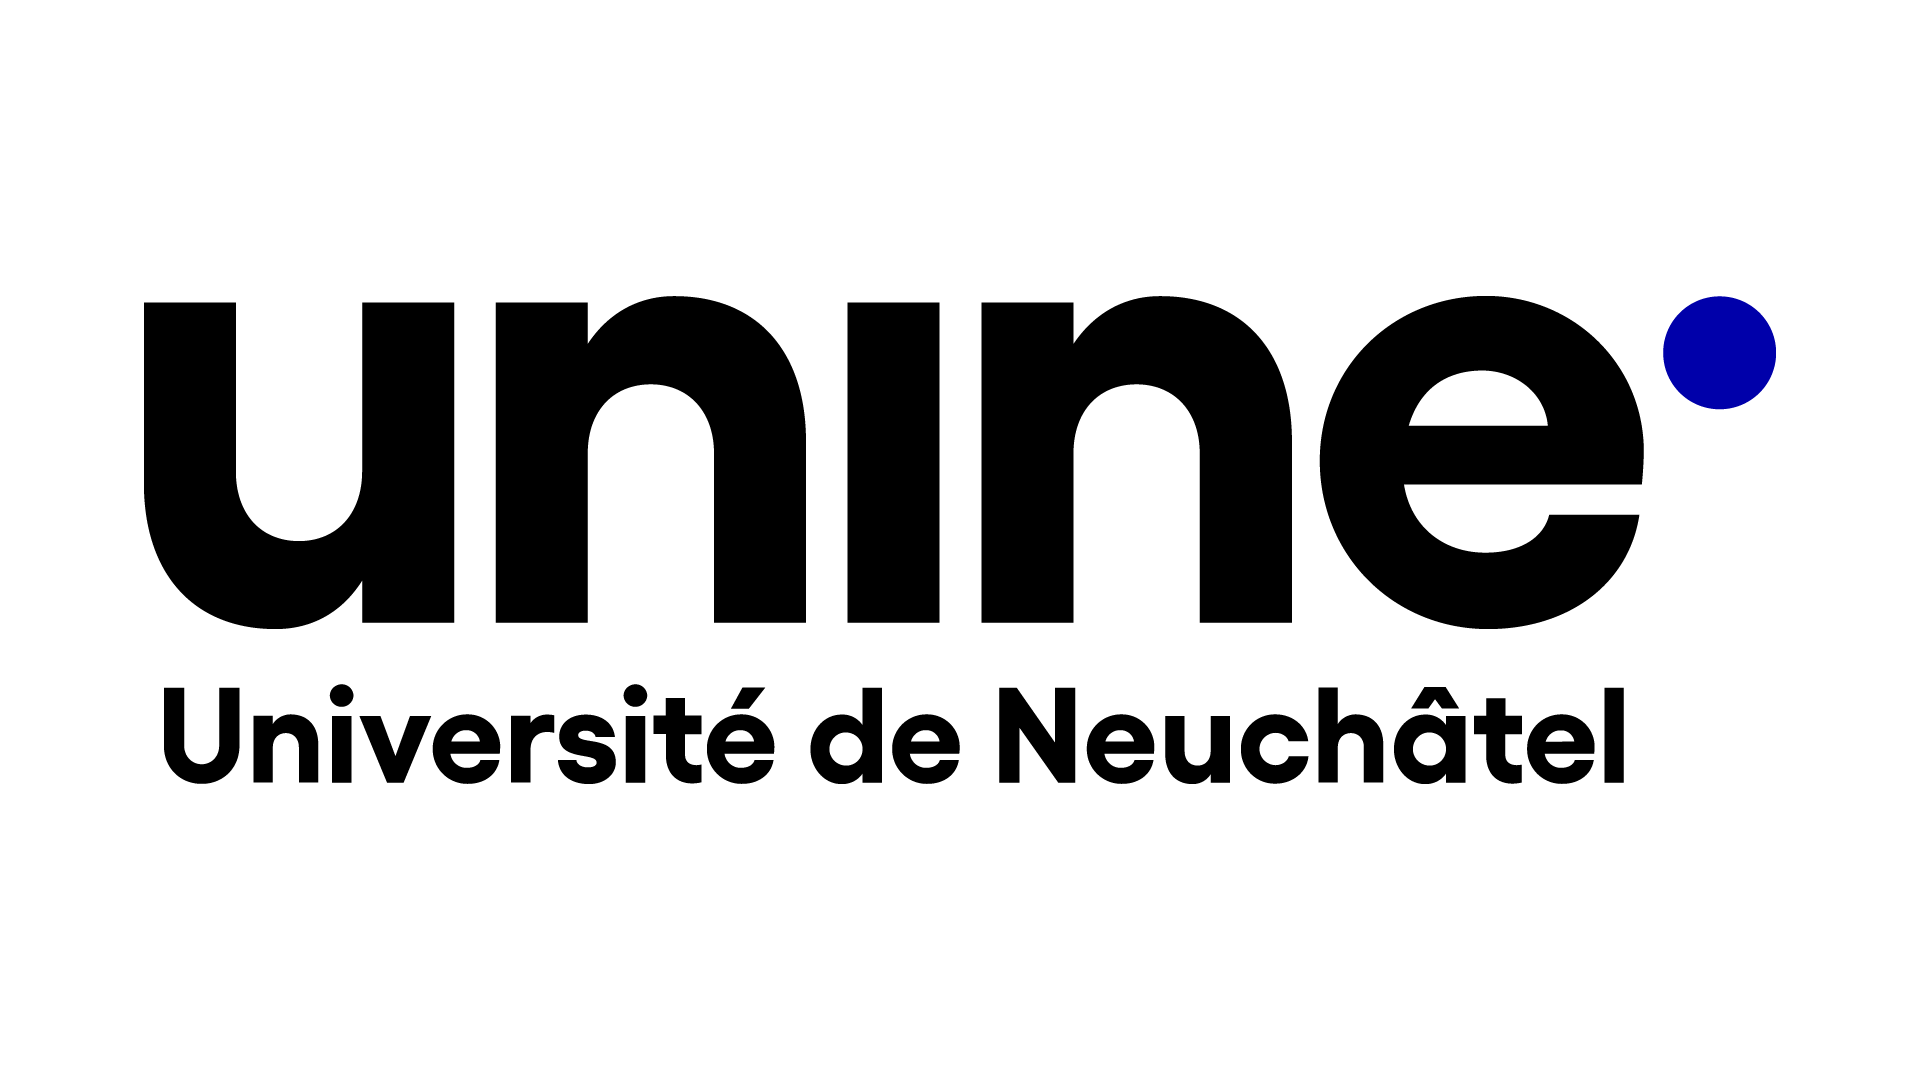
\includegraphics[width=0.17\textwidth,keepaspectratio]{figures/unine_logo.png}
\end{tabular}
\end{center}

\vspace*{4.1cm}

\begin{center}
{\Large Reproducing and Extending Nash Regret Experiments}\\[0.18cm]
{\Large in Zero-Sum Matrix Games}\\[0.75cm]

{\large Project Report}\\[0.35cm]

{\normalsize Based on the paper}\\[0.18cm]
{\itshape On the Limitations and Possibilities of Nash Regret Minimization}\\
{\itshape in Zero-Sum Matrix Games Under Noisy Feedback}\\[0.95cm]

{\large Bill Chavez}\\[-0.02cm]
{\normalsize \texttt{bill.chavezarias@students.unibe.ch}}\\[0.36cm]

{\large Mateo Lopez}\\[-0.02cm]
{\normalsize \texttt{mateo.lopez@unine.ch}}\\[0.36cm]

{\large Felix Merz}\\[-0.02cm]
{\normalsize \texttt{felix.merz@students.unibe.ch}}\\[0.36cm]

{\large Daksh Patel}\\[-0.02cm]
{\normalsize \texttt{daksh.patel@students.unibe.ch}}\\[0.65cm]

{\small \url{https://github.com/MateoLopez00/Zero-Sum-MatrixGames.git}}
\end{center}

\vfill

\noindent
\begin{tabular}{@{}p{0.34\textwidth}p{0.62\textwidth}@{}}
\textbf{Date:} & Spring 2026 \\[0.10cm]
\textbf{Course:} & Seminar Advanced Topics in Reinforcement Learning and Decision Making \\[0.10cm]
\end{tabular}

\restoregeometry
\end{titlepage}

\pagestyle{plain}
\pagenumbering{arabic}

\section*{Abstract}

This report reproduces and extends the empirical study of Nash regret minimisation in zero-sum matrix games under noisy feedback by Maiti, Jamieson and Ratliff~\cite{maiti2023nashregret}. We reproduce the paper's full-information diagonal-game experiments and its $2\times2$ bandit experiments, then study bilateral learning, Gaussian noise robustness, and a beyond-$2\times2$ bandit stress test. The reproduced settings show the expected flatter regret growth for the proposed algorithms relative to generic baselines. The extensions identify which assumptions matter: noise-aware delays help in the full-information game, the original bandit algorithm remains the relevant noisy Section 4 comparison, bilateral learning changes the opponent model, and larger bandit games expose limits outside the proved $2\times2$ regime. The report states horizons, seeds, run counts, game sizes, adversaries, and noise levels to support reproducibility.

\section{Introduction}

Nash regret minimisation in zero-sum matrix games studies whether a learner can maintain payoffs close to the value of the game while facing a strategic or adversarial column player. The source paper~\cite{maiti2023nashregret} shows that this is possible in selected feedback models, but also that generic bandit or online-learning methods can fail under adversarial play.

Our project has five contributions: reproducing Section 3 full-information experiments; reproducing Section 4 bandit experiments; studying bilateral learning; testing Gaussian noise robustness; and applying the Section 4 bandit construction to larger diagonal games outside the proved $2\times2$ regime.

The report is organized as follows. Section 2 defines games, feedback models, algorithms, adversaries, and the regret metric. Section 3 gives the exact experimental settings and reproduction results. Sections 4--6 present the three extensions. Section 7 discusses reproducibility, limitations, and the conclusions supported by the experiments.

\section{Models, Metrics, and Assumptions}

\subsection{Zero-sum matrix games and Nash regret}

Let $A\in[0,1]^{m\times n}$ be the row player's payoff matrix. For mixed strategies $x$ and $y$, the expected payoff is $x^\top A y$, and the value of the zero-sum game is
\[
  \Vstar=\max_x \min_y x^\top A y.
\]
At round $t$, the row learner plays $x_t$ and the column player chooses $y_t$ according to a fixed rule or adversary. We report cumulative Nash regret
\[
  \Reg_T=\sum_{t=1}^T \left(\Vstar - x_t^\top A y_t\right),
\]
with the sign convention used in the implementation: smaller cumulative regret indicates that the row learner remains closer to the game value.

\newpage
\subsection{Feedback models}

The project uses three feedback models. In the Section 3 full-information setting, the learner observes a full payoff signal on a diagonal game with
$A_{ii}=0.4+0.2(i-1)/(n-1)$ and $n\in\{10,20,50,100\}$. In the Section 4 bandit setting, the learner observes only the played cell in the $2\times2$ game
\[
  A=\begin{pmatrix}2/3&0\\0&1/3\end{pmatrix},\qquad \Vstar=2/9.
\]
In the Gaussian-noise extension, a full-information observation is clipped to $[0,1]$ after adding Gaussian noise entrywise, while the bandit version observes only
\[
  \operatorname{clip}\!\left(A_{i_tj_t}+\sigma Z_t,0,1\right),\qquad Z_t\sim\mathcal{N}(0,1).
\]
This clipping assumption keeps payoffs bounded but can bias observations near 0 and 1; therefore noisy-extension curves are not expected to match noiseless curves numerically.

\subsection{Algorithms and baselines}

The full-information experiments compare an empirical Nash baseline, Hedge, and the paper's proposed algorithm. Hedge is a standard expert-advice method~\cite{freund1997decision,cesabianchi2006prediction}. The bandit experiments compare UCB, EXP3, and \OurAlg{}. UCB is a stochastic-bandit baseline~\cite{auer2002finite}, while EXP3 is the standard adversarial-bandit baseline~\cite{auer2002nonstochastic}. The noise-aware full-information variant modifies only the update delay of the proposed method; the Section 4 noise experiments keep the original bandit \OurAlg{} rather than adding a separate noise-aware variant.

\subsection{Adversaries and assumptions}

Each Section 4 trial has two phases of length $T/2$. Phase 1 uses one of the three adversaries from the paper: threshold best response, tolerance-band best response, or fixed Nash play $(1/3,2/3)$. Phase 2 always uses pure best response. The Section 4 noise extension keeps exactly these adversaries and phases; only the observation channel changes. All results are finite-horizon Monte Carlo estimates rather than asymptotic proofs.

\section{Reproduction Methodology and Results}

Figure~\ref{fig:baseline} summarises the two reproduction experiments using cumulative regret curves. Table~\ref{tab:settings} gives the exact settings used for the report figures and tables. Short source identifiers are used in the table to avoid unreadable path overflow; the identifiers refer to the notebooks and scripts listed in the final paragraph of this section. Figures are copied into \texttt{Final\_report/figures} only to make the LaTeX package self-contained; the experiments themselves are regenerated from the original notebooks and scripts.

\begin{table}[!htbp]
  \centering
  \scriptsize
  \setlength{\tabcolsep}{4pt}
  \renewcommand{\arraystretch}{0.86}
  \begin{tabularx}{\textwidth}{p{0.19\textwidth}X p{0.18\textwidth}}
    \toprule
    Experiment & Reported settings & Source \\
    \midrule
    Section 3 reproduction & Diagonal games $n\in\{10,20,50,100\}$; cumulative Nash regret; $T=100{,}000$; six seeds; algorithms: Nash, Hedge, Our-Algo. & S3 curves \\
    Section 4 reproduction & $2\times2$ game with $\Vstar=2/9$; adversaries 1--3; two phases of $T/2$; $T=100{,}000$; 32 seeds; algorithms: UCB, EXP3, OurAlg. & S4 curves \\
    Section 3 noise & Full-information Gaussian-clipped feedback; $n=100$ convergence plots; $\sigma\in\{0.1,0.2,0.3\}$; $T=100{,}000$; 12 runs; seed 7. & S3 noise \\
    Section 4 noise & Same Section 4 adversaries and phases; played-cell Gaussian-clipped feedback; $\sigma\in\{0.1,0.2,0.3\}$; $T=100{,}000$; 32 runs; seed 42. & S4 noise \\
    Bilateral learning & Both players update rather than fixing the column rule; diagonal full-information game shown at $n=30$; $2\times2$ bandit game shown with bilateral learner pairs only. & Bilateral \\
    Beyond $2\times2$ & Diagonal bandit games $n\in\{2,3,4,5,7,10\}$; $T$ up to $10^6$; 128 trials; algorithms: UCB, EXP3, OurAlg. & S4 larger-$n$ \\
    \bottomrule
  \end{tabularx}
  \caption{Reproducibility settings used in the report. These are scientific settings, not internal code preset labels.}
  \label{tab:settings}
\end{table}

\begin{figure}[!htbp]
  \centering
  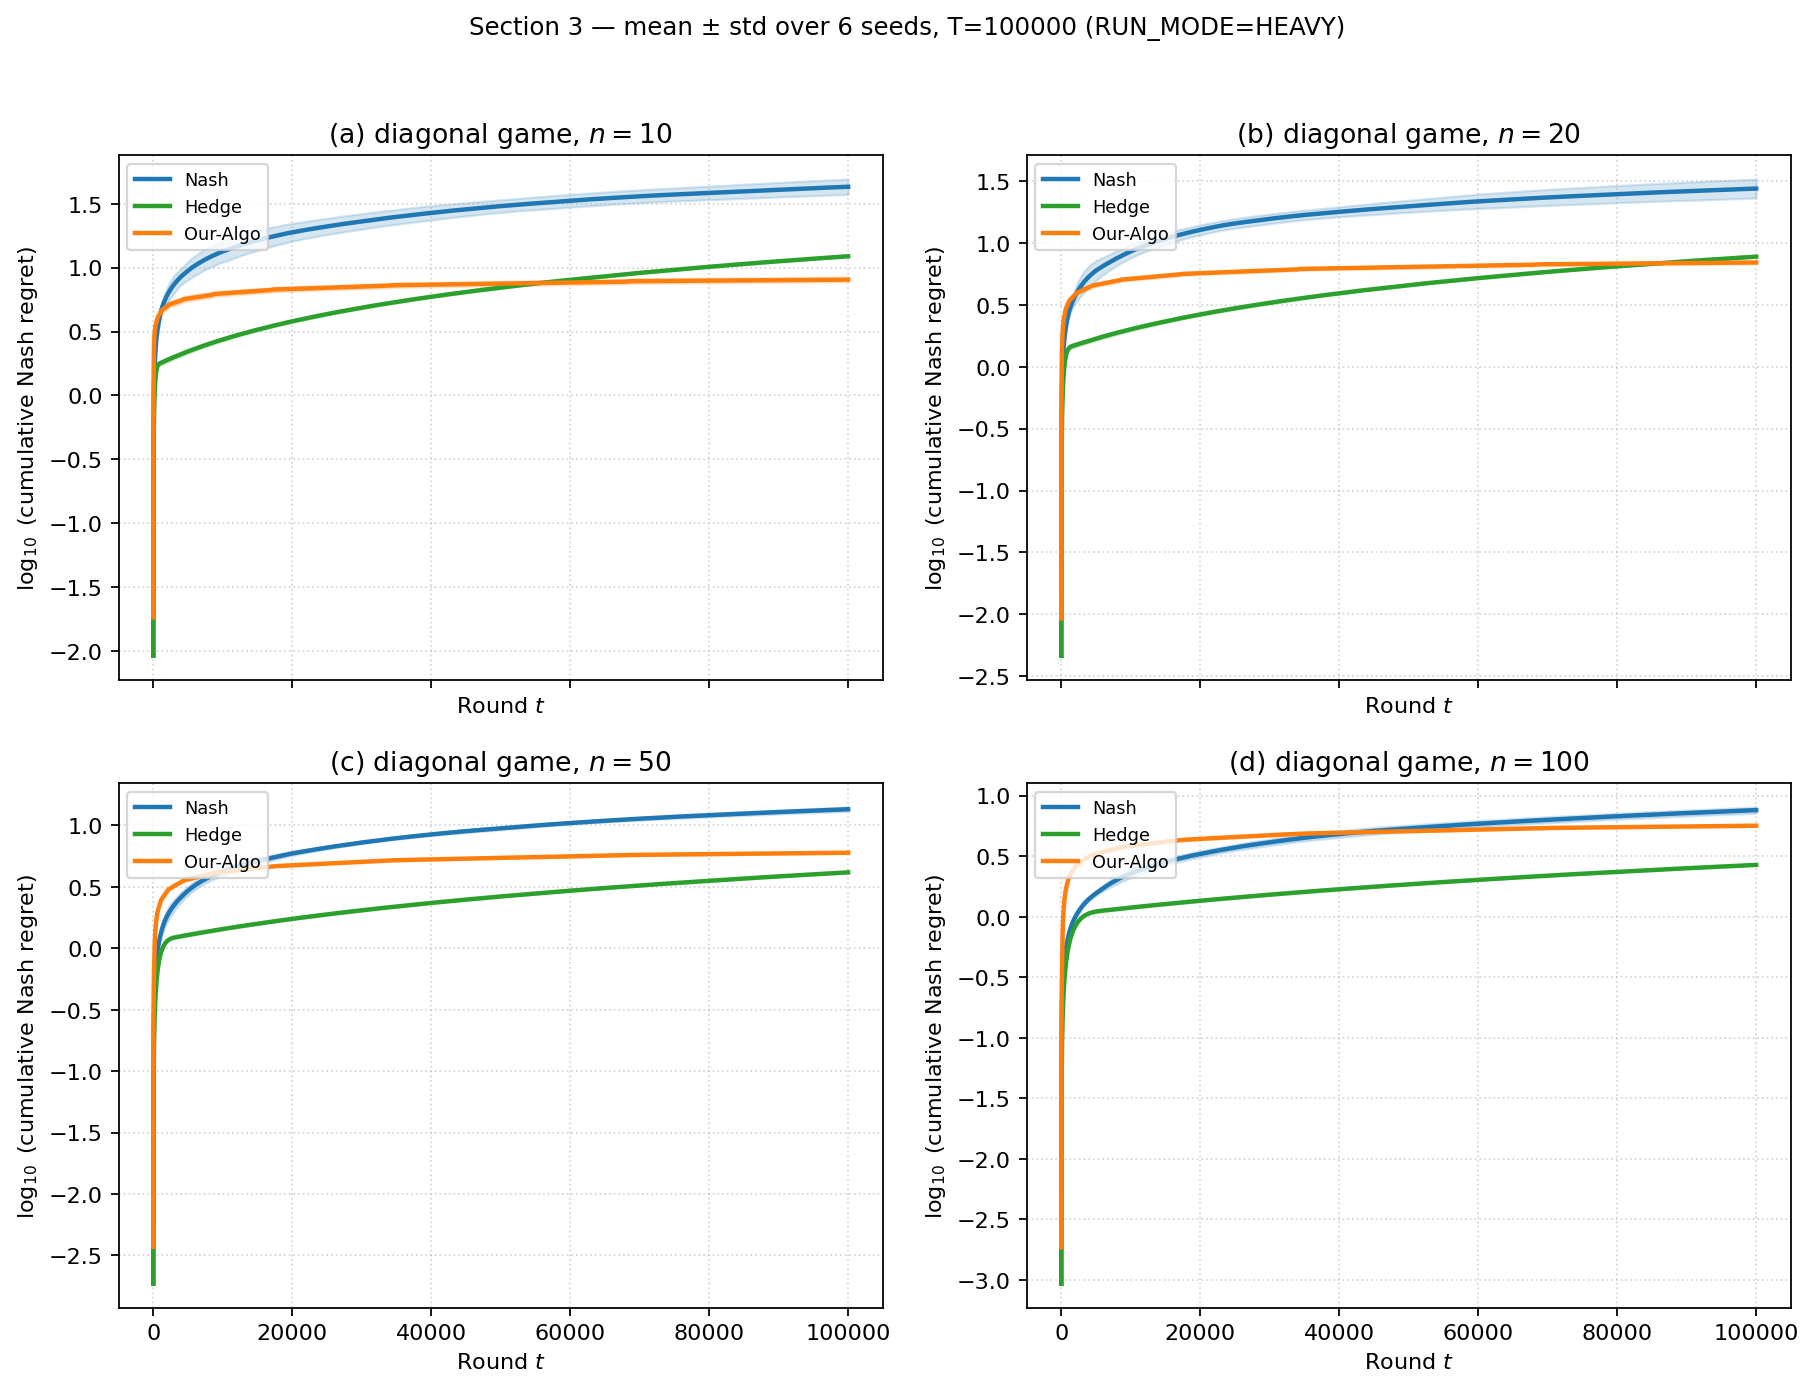
\includegraphics[width=0.82\textwidth]{figures/section3_baseline_cumulative_T100000.png}

  \vspace{0.04cm}
  {\small (a) Section 3 full-information diagonal games.}

  \vspace{0.08cm}

  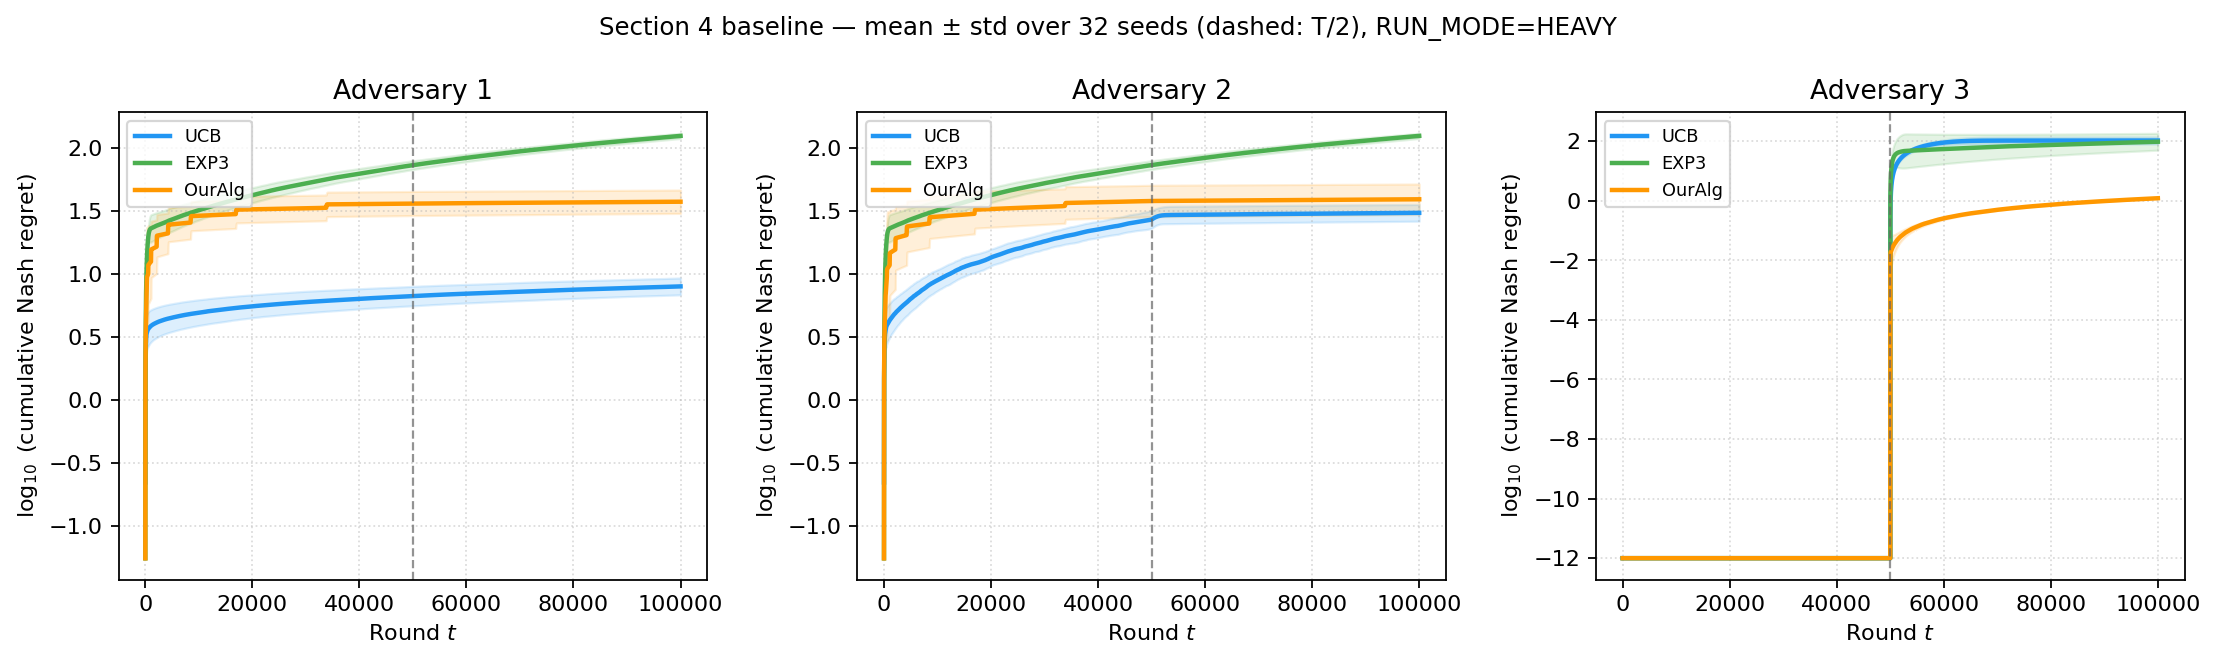
\includegraphics[width=0.82\textwidth]{figures/section4_baseline_cumulative_T100000.png}

  \vspace{0.04cm}
  {\small (b) Section 4 bandit adversaries.}

  \caption{Reproduction cumulative Nash-regret curves at $T=100{,}000$. Panel (a) shows the Section 3 full-information diagonal games; panel (b) shows the Section 4 two-phase bandit adversaries.}
  \label{fig:baseline}
\end{figure}

The reproduction is technically consistent with the paper's assumptions. In the full-information setting, the strongest qualitative signal is not a single terminal value but the curve shape: the proposed algorithm pays an early exploration cost and then slows, while the baselines keep accumulating regret more steadily, especially for smaller diagonal games. In the bandit setting, the adversarial phase structure is crucial. Adversary 3 is benign in Phase 1 because it plays Nash, but the Phase 2 best response sharply separates algorithms. This matches the theoretical motivation: generic UCB and EXP3 are not designed for this adversarial game protocol, while \OurAlg{} uses the structure of the $2\times2$ matrix game.

For provenance, S3 curves are generated by the Section 3 Nash-regret curves notebook, S4 curves by the Section 4 Nash-regret curves notebook, S3/S4 noise by the two noise-robustness notebooks, S4 larger-$n$ by the beyond-$2\times2$ notebook, and bilateral learning by the two bilateral scripts. These source names are intentionally summarized here; the repository structure contains the exact files and copied figures.

\section{Noise Robustness Extension}

The main extension tests a controlled change in the feedback model. For Section 3, we add Gaussian noise to the full-matrix feedback and clip entries into $[0,1]$. For Section 4, only the played bandit cell is observed as
\[
  \operatorname{clip}\!\left(A_{i_tj_t}+\sigma Z_t,0,1\right),\qquad Z_t\sim\mathcal{N}(0,1).
\]
Clipping is an important modelling assumption: it keeps payoffs in range but can bias observations near 0 and 1. Therefore the noisy-extension curves should not be expected to numerically reproduce the noiseless Section 4 curves.

\paragraph{Full-information noise-aware variant.}
The baselines remain unchanged. The extension modifies only the paper's algorithm by delaying updates more when feedback is noisier:
\[
  \tau_{\text{orig}}=\min\{\log^2(T),\sqrt{T}\},\qquad
  \tau_{\text{noise}}=\min\{(1+2\sigma)\log^2(T),\sqrt{T}\}.
\]
The experiment uses $T=100{,}000$, $n=100$ for the convergence plots, 12 independent runs, seed 7, and $\sigma\in\{0.1,0.2,0.3\}$. Table~\ref{tab:s3noise} reports terminal regret at $\sigma=0.3$ over the diagonal games used in the sweep.

\begin{table}[!htbp]
  \centering
  \small
  \begin{tabular}{rrrrrr}
    \toprule
    $n$ & Nash & Hedge & Our-Algo & Noise-aware & Reduction \\
    \midrule
    10 & 113.08 & 16.30 & 8.54 & 8.25 & 3.4\% \\
    20 & 58.66 & 15.48 & 6.36 & 6.08 & 4.4\% \\
    50 & 24.41 & 15.33 & 5.02 & 4.78 & 4.8\% \\
    100 & 12.99 & 15.75 & 4.58 & 4.30 & 6.1\% \\
    \bottomrule
  \end{tabular}
  \caption{Section 3 noise robustness at $\sigma=0.3$, $T=100{,}000$, 12 runs. The reduction is relative to the original Our-Algo.}
  \label{tab:s3noise}
\end{table}

\begin{figure}[!htbp]
  \centering
  \begin{minipage}{0.315\textwidth}
    \centering
    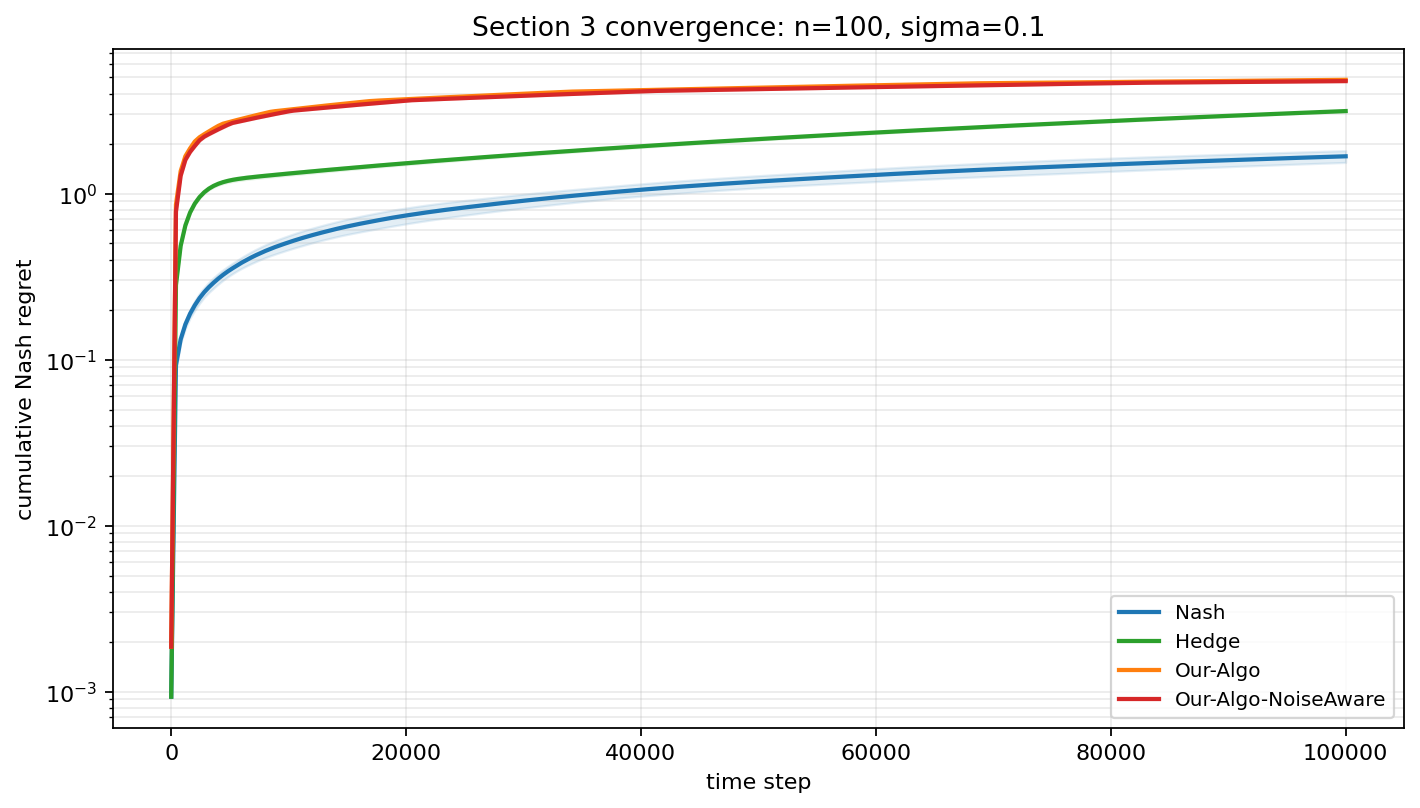
\includegraphics[width=\linewidth]{figures/section3_noise_n100_sigma0p1.png}\\
    {\small (a) $\sigma=0.1$}
  \end{minipage}\hfill
  \begin{minipage}{0.315\textwidth}
    \centering
    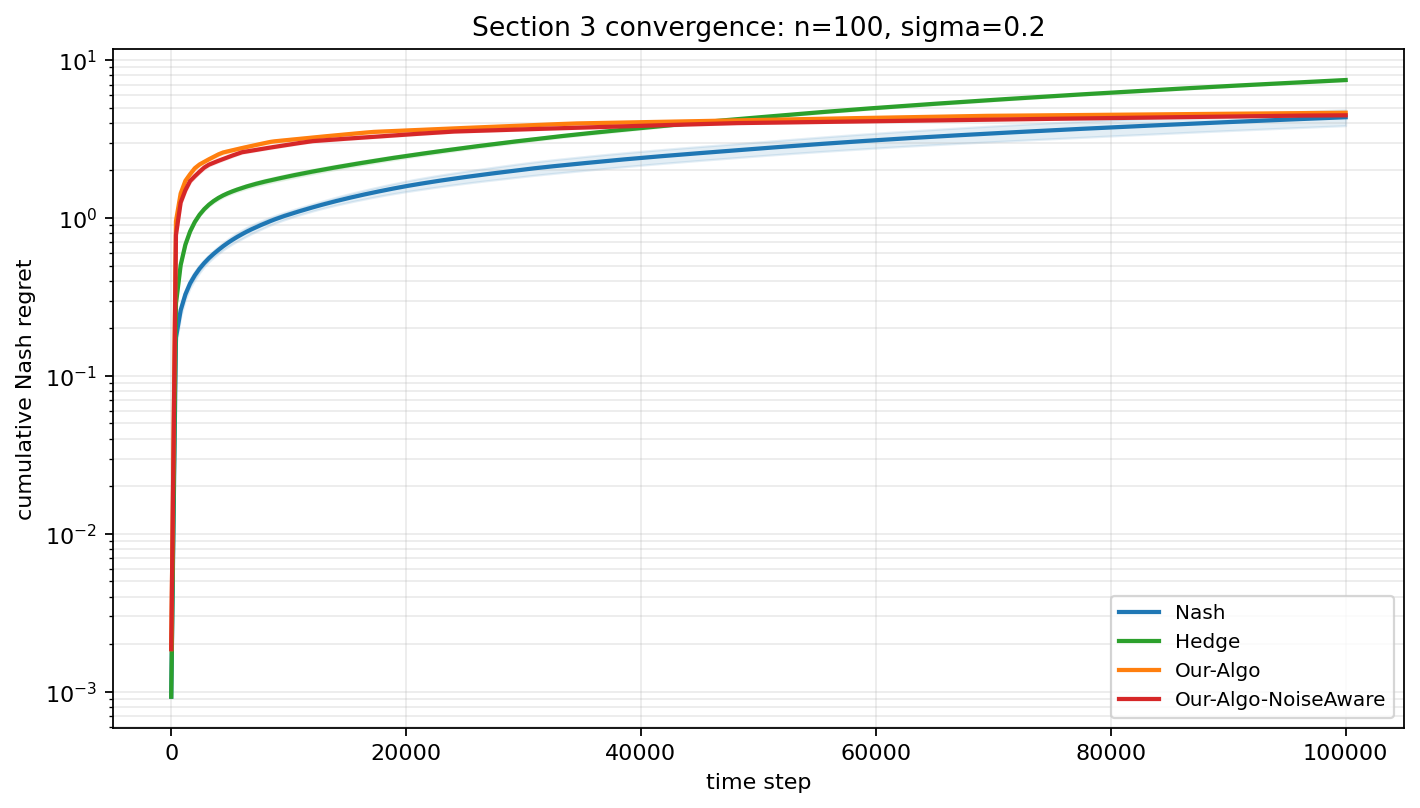
\includegraphics[width=\linewidth]{figures/section3_noise_n100_sigma0p2.png}\\
    {\small (b) $\sigma=0.2$}
  \end{minipage}\hfill
  \begin{minipage}{0.315\textwidth}
    \centering
    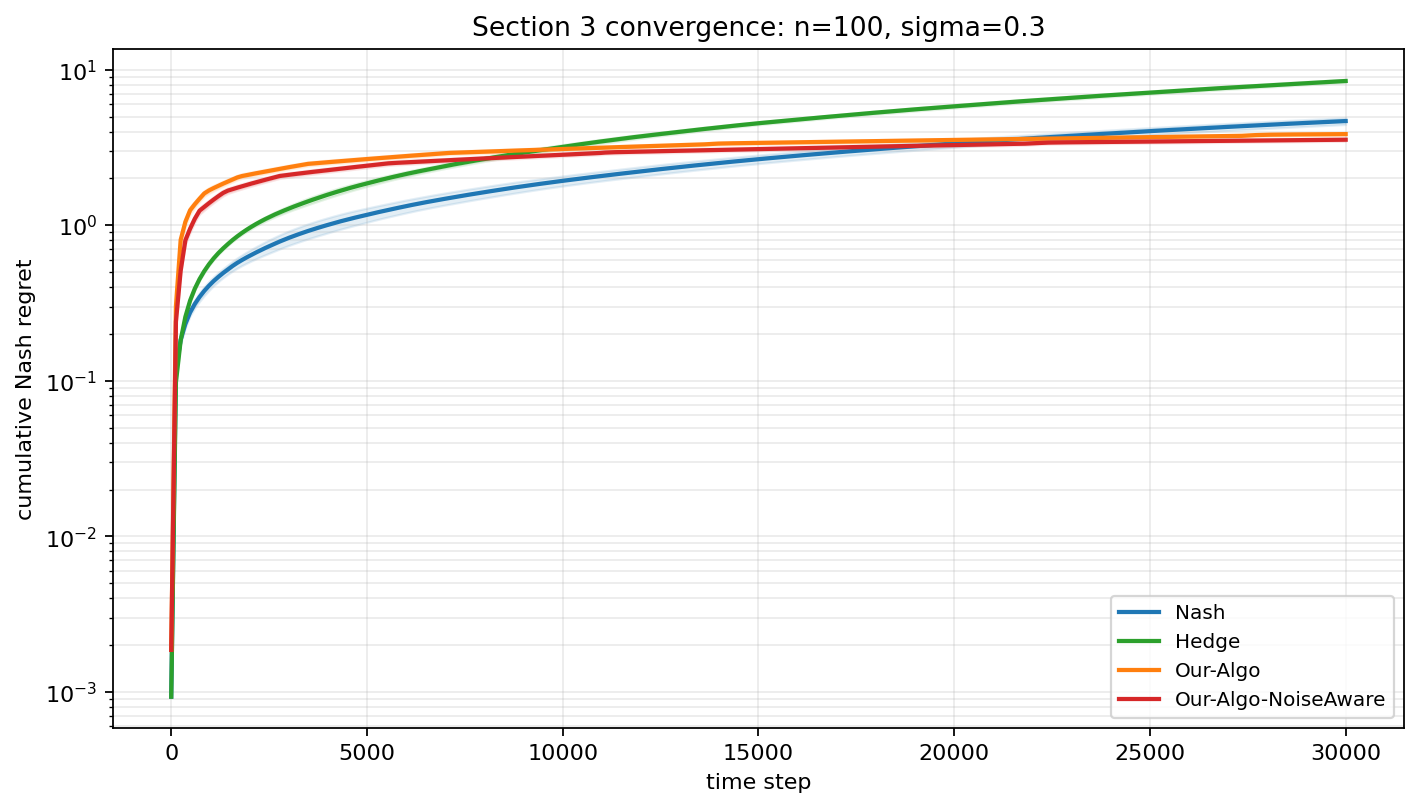
\includegraphics[width=\linewidth]{figures/section3_noise_n100_sigma0p3.png}\\
    {\small (c) $\sigma=0.3$}
  \end{minipage}
   \caption{Section 3 noise convergence for $n=100$ and $T=100{,}000$. The noise-aware variant becomes more useful as $\sigma$ increases.}
  \label{fig:s3noise}
\end{figure}

The result supports the intended mechanism. When $\sigma$ is small, the empirical matrix is reliable enough that the extra delay has little effect, and Nash can still be competitive at $n=100$. At higher noise, premature updates based on noisy estimates become more costly, while the two proposed variants flatten relative to Nash and Hedge. The improvement from the noise-aware threshold is moderate rather than dramatic, which is also an important caveat: the original method is already robust in this setting.

\paragraph{Bandit noise with the same adversaries.}
For Section 4, we do not introduce a noise-aware bandit variant in the final comparison. The adversaries and two-phase protocol are exactly the same as in the reproduction: the extension imports the same adversary logic from \texttt{section4\_bandit.py}. The only change is the feedback distribution, from Bernoulli observations to clipped Gaussian played-cell observations. The reported runs use $T=100{,}000$, 32 independent runs, seed 42, and $\sigma\in\{0.1,0.2,0.3\}$.

\begin{table}[!htbp]
  \centering
  \small
  \begin{tabular}{rrrr}
    \toprule
    Adversary & UCB & EXP3 & OurAlg \\
    \midrule
    1 & 7.53 & 141.27 & 77.90 \\
    2 & 59.01 & 140.74 & 86.07 \\
    3 & 778.26 & 703.05 & 2.86 \\
    \bottomrule
  \end{tabular}
  \caption{Final Section 4 Nash regret at $\sigma=0.3$, $T=100{,}000$, 32 runs.}
  \label{tab:s4noise}
\end{table}

\begin{figure}[H]
  \centering
  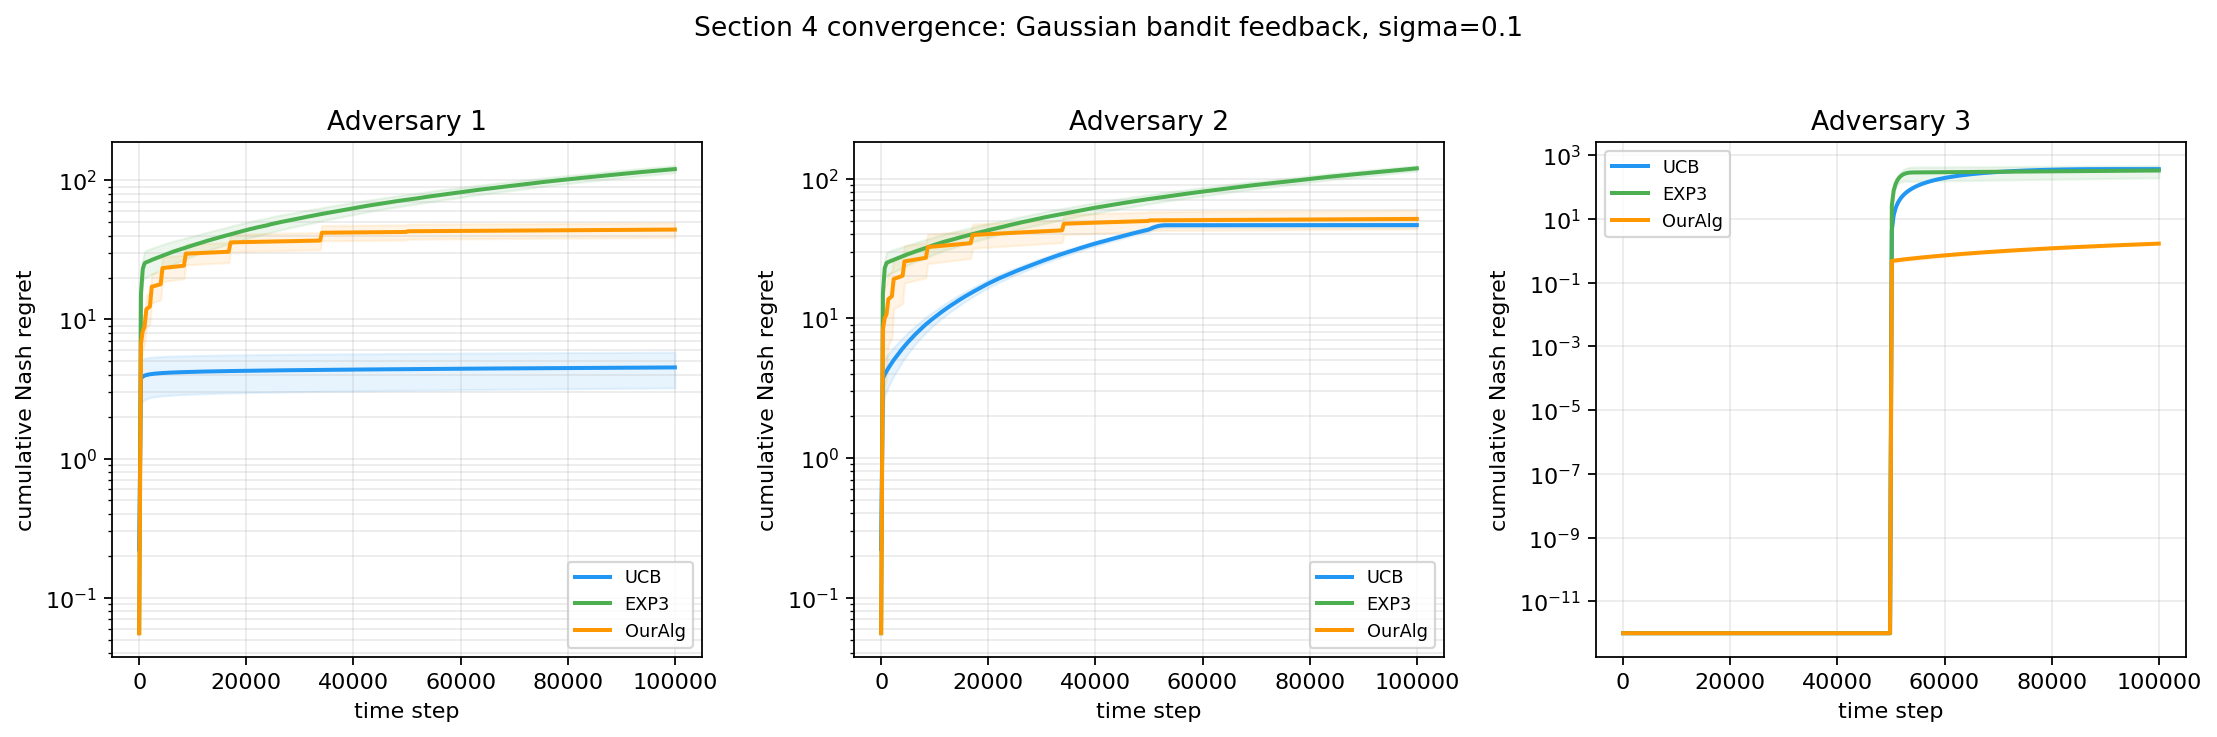
\includegraphics[width=0.82\textwidth]{figures/section4_noise_sigma0p1.png}

  \vspace{0.04cm}
  {\small (a) $\sigma=0.1$}

  \vspace{0.10cm}

  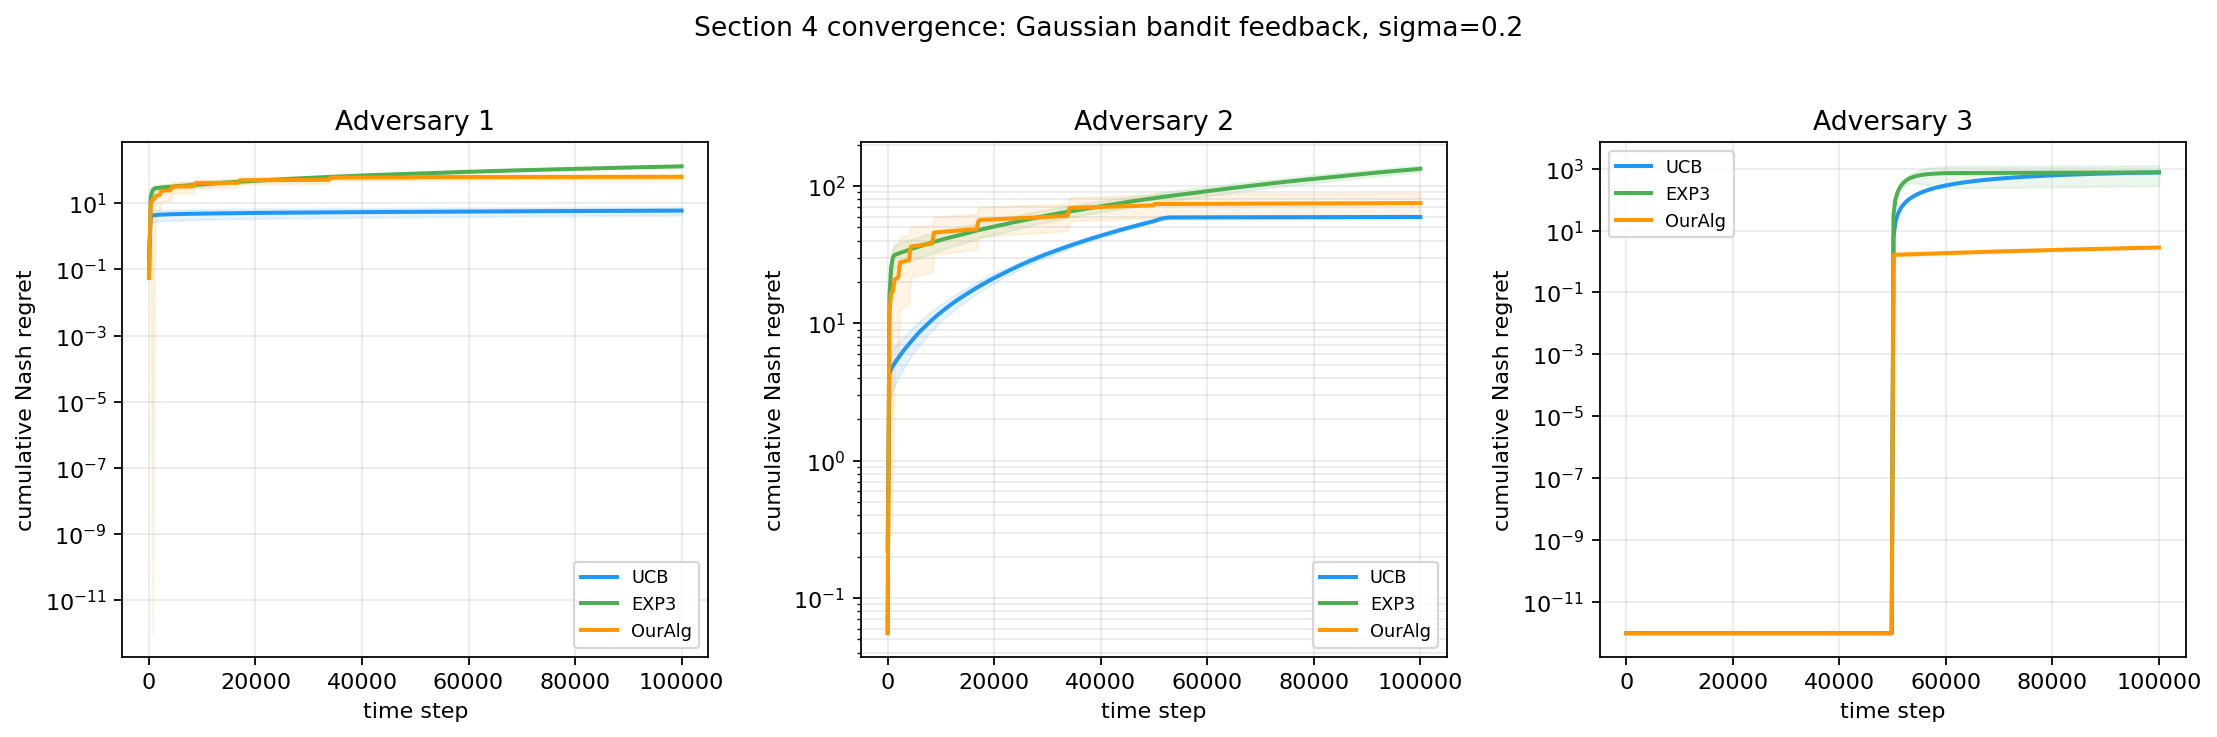
\includegraphics[width=0.82\textwidth]{figures/section4_noise_sigma0p2.png}

  \vspace{0.04cm}
  {\small (b) $\sigma=0.2$}

  \vspace{0.10cm}

  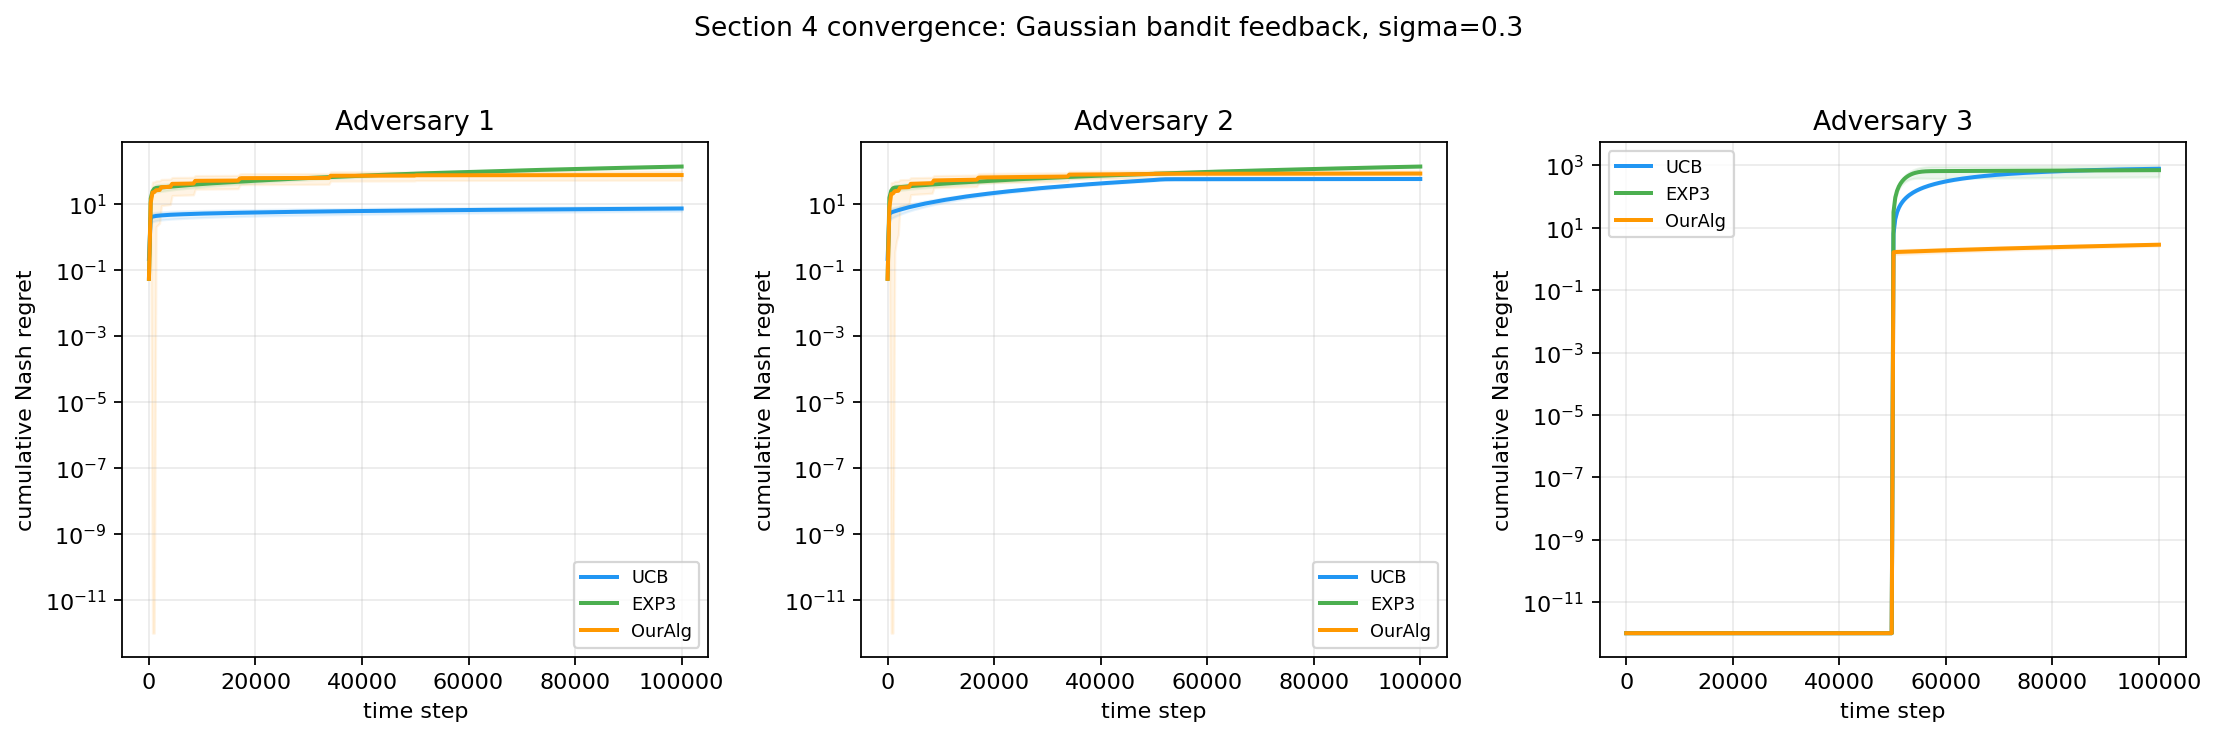
\includegraphics[width=0.82\textwidth]{figures/section4_noise_sigma0p3.png}

  \vspace{0.04cm}
  {\small (c) $\sigma=0.3$}

  \caption{Section 4 noisy bandit convergence, $T=100{,}000$. Each row contains Adversaries 1--3 for one noise level.}
  \label{fig:s4noise}
\end{figure}

The bandit extension should be interpreted relative to its modified feedback channel. Since clipped Gaussian samples have different variance and bias properties from Bernoulli observations, rankings need not match the noiseless Figure 2 reproduction. The most stable qualitative finding is on Adversary 3: at high noise, UCB and EXP3 accumulate very large regret after the phase switch, whereas \OurAlg{} remains close to the game value. Against Adversaries 1 and 2, rankings are more adversary-dependent: UCB can remain competitive, EXP3 is usually the largest-regret baseline, and \OurAlg{} sits between them in these noisy finite-horizon runs.

\FloatBarrier

\section{Bilateral Learning Extension}

The paper evaluates a row learner against a fixed or adversarial column rule. 
Our bilateral extension changes this setting by allowing both players to update 
their strategies simultaneously from feedback. This constitutes a different 
learning scenario rather than a simple parameter variation, since the standard 
best-response regret interpretation no longer directly applies in self-play. 
In particular, the instantaneous payoff 
$ x_t^\top A y_t $ 
may exceed the equilibrium value 
$ V^\star $, 
making the signed equilibrium gap negative.

Instead of reporting signed regret, we measure the cumulative absolute equilibrium gap

\[
\sum_{t=1}^T \left| V^\star - x_t^\top A y_t \right|,
\]

which serves as a stability metric indicating whether the joint dynamics converge 
toward the Nash equilibrium value over time.

In the full-information diagonal game, both players observe sampled matrix entries 
and run pairings such as \OurAlg{}--\OurAlg{}, Hedge--Hedge, Nash--Nash, and mixed pairs. 
In the $2 \times 2$ bandit game, both players use bandit-feedback updates on the 
same matrix game as in the Section~4 reproduction.

\begin{figure}[!htbp]
  \centering
  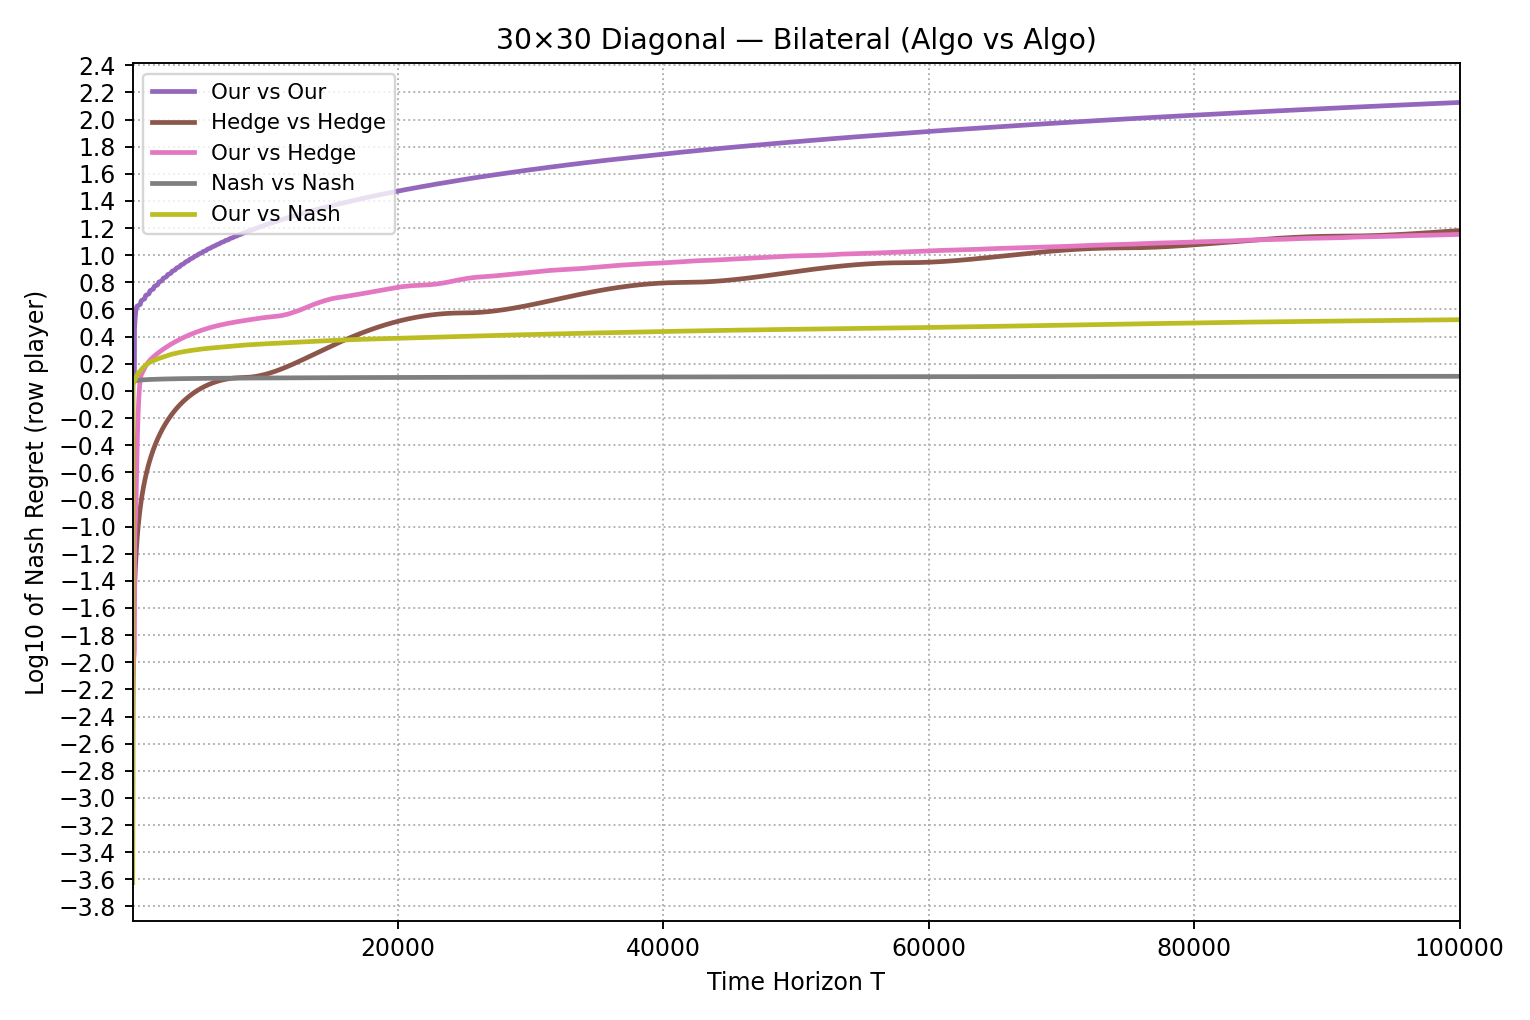
\includegraphics[width=0.78\textwidth]{figures/section3_bilateral_n30.png}

  \vspace{0.15cm}
  {\small (a) Section 3 diagonal game, $n=30$.}

  \vspace{0.40cm}

  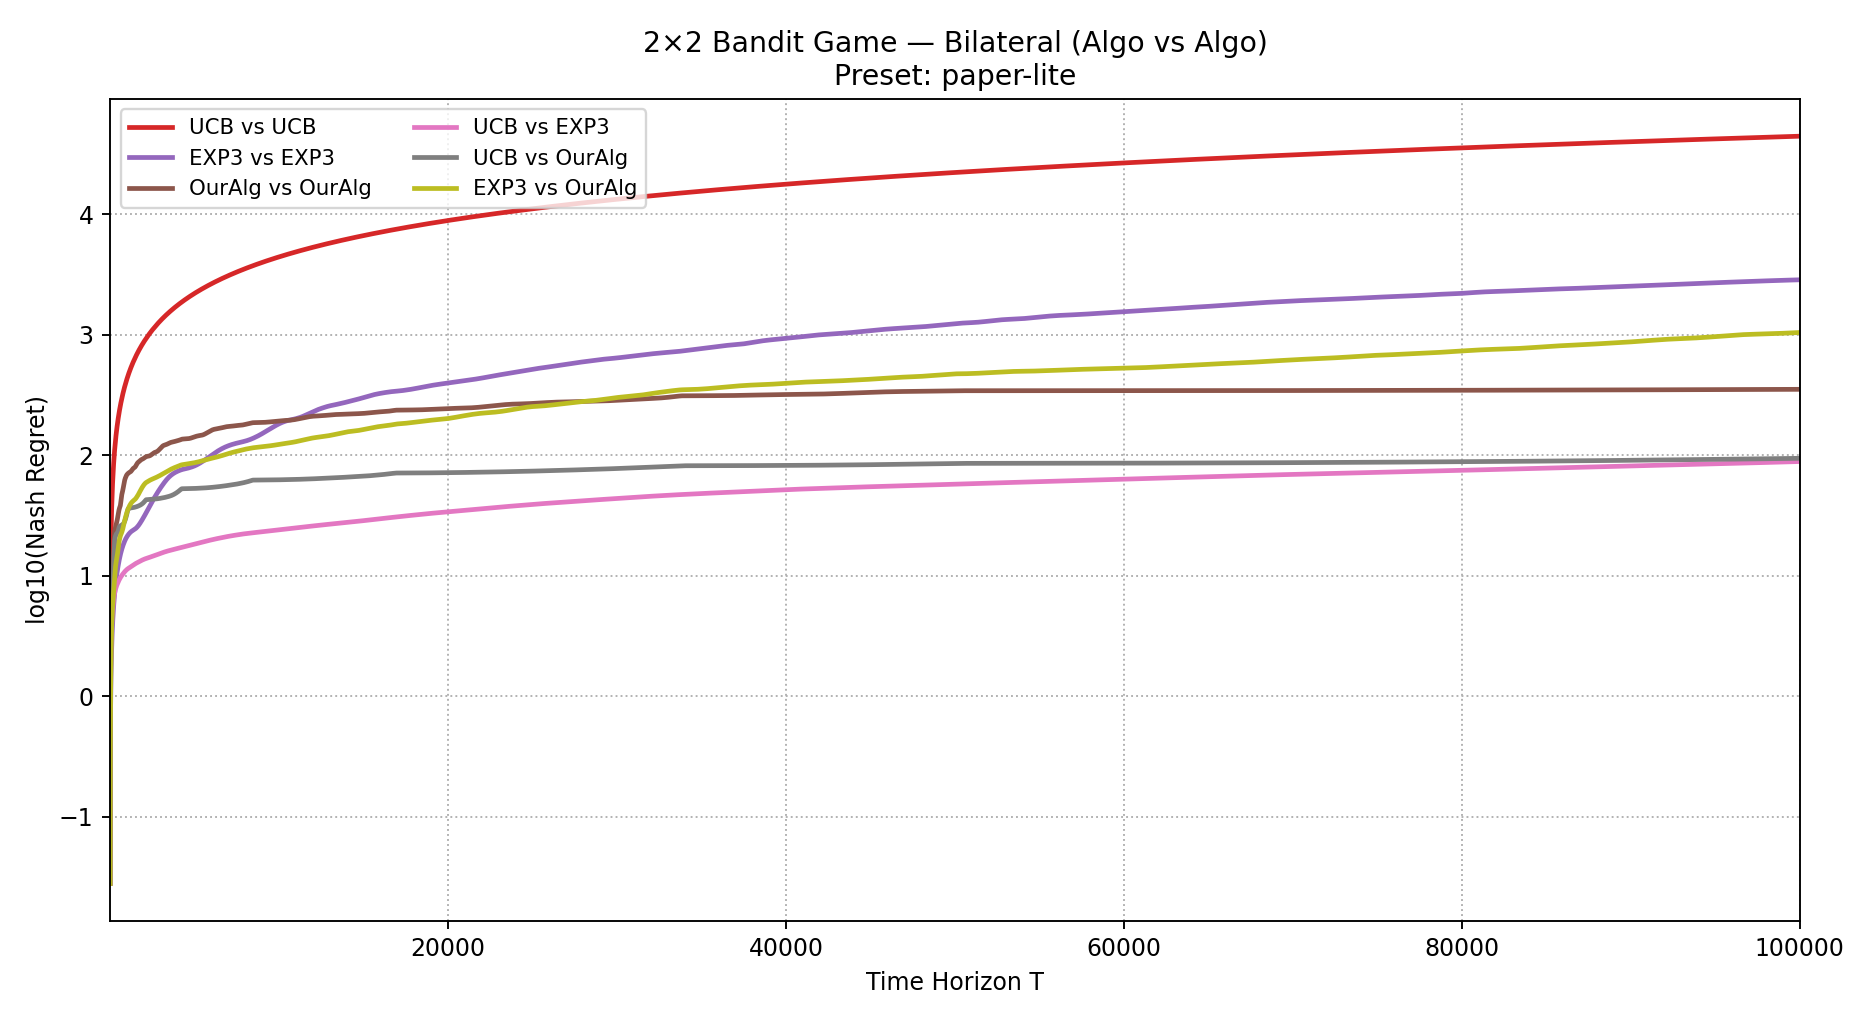
\includegraphics[width=0.88\textwidth]{figures/section4_bilateral_paper_lite.png}

  \vspace{0.15cm}
  {\small (b) Section 4 bandit game.}

  \caption{Bilateral-learning extension. Both panels show learner-vs-learner curves only: full-information diagonal-game pairings in panel (a), and $2\times2$ bandit pairings in panel (b).}
  \label{fig:bilateral}
\end{figure}

The results should not be interpreted as contradicting the original paper when 
they differ from the adversarial baseline, since the opponent model changes 
fundamentally in the bilateral setting.

In the Section~3 experiment, Nash--Nash remains nearly flat because both players 
repeatedly play the empirical Nash equilibrium of their current estimates, which 
keeps the observed payoff close to $V^\star$ from early rounds onward and avoids 
large exploratory deviations. In contrast, \OurAlg{}--\OurAlg{} exhibits the 
largest cumulative absolute equilibrium gap because \OurAlg{} includes an aggressive 
warm-up and reinitialization phase. When both players simultaneously explore in 
this manner, the joint dynamics initially drift farther from $V^\star$ before 
eventually stabilizing. Mixed pairings such as \OurAlg{}--Nash and 
\OurAlg{}--Hedge lie between these extremes, reflecting the interaction between 
an exploratory row learner and a more stable column strategy.

In Section~4, UCB--UCB produces the largest growth because UCB was originally 
designed for single-agent stochastic optimization rather than simultaneous 
equilibrium learning. The optimistic updates of the row player and pessimistic 
updates of the column player can induce persistent oscillatory behavior, delaying 
convergence toward the Nash value. EXP3--EXP3 also accumulates a large equilibrium 
gap because EXP3 maintains persistent exploration throughout the horizon. 
By comparison, \OurAlg{}--\OurAlg{} plateaus at a lower level than both baselines, 
suggesting that its update structure is more compatible with bilateral convergence 
in the $2 \times 2$ setting.

Overall, these experiments indicate that bilateral learning introduces a distinct 
dynamical regime compared with the original adversarial formulation. The setting 
is therefore useful for studying adaptive multi-agent interaction, although it 
falls outside the assumptions of the original regret analysis, which considers 
a fixed adversarial column player rather than a simultaneously adapting opponent.

\FloatBarrier

\section{Non-Adversarial Column Player Extension}
The algorithm Arnab et al. minimizes the regret against an adversarial column player, but how does the algorithm react when the column player is not deliberately trying to minimize the row player's return? This extension explores how the algorithm from Arnab et al. adapts to less hostile and presumably easier environments.

We use three non-adversarial responses, a fixed response, a uniform response, and a random response. A fixed response is a response where the column player plays the same action in every round. Uniform response means the column player always plays the strategy that gives equal probability to each action, specifically $y_t=\frac{1}{m}\mathbf{1}, \; \forall t \in T$. For the random response you draw a new, random simplex in each round using the Dirichlet distribution, which will then serve as the column player's strategy.

The Nash regret is used to evaluate the performance, like in the adversarial scenario. Thus, the results allow a direct comparison between the alternative scenarios.

The algorithm from Arnab et al. still achieves sub-polynomial regret against these weaker opponents, see Fig. \ref{fig:non-adversarial}. The row player incures substatially less regret than he does against an adversarial coloumn player. This affirms the paper's claim that their algorithm achieves polylog(T) regret against any player. 

\begin{figure}[!htbp]
  \centering
  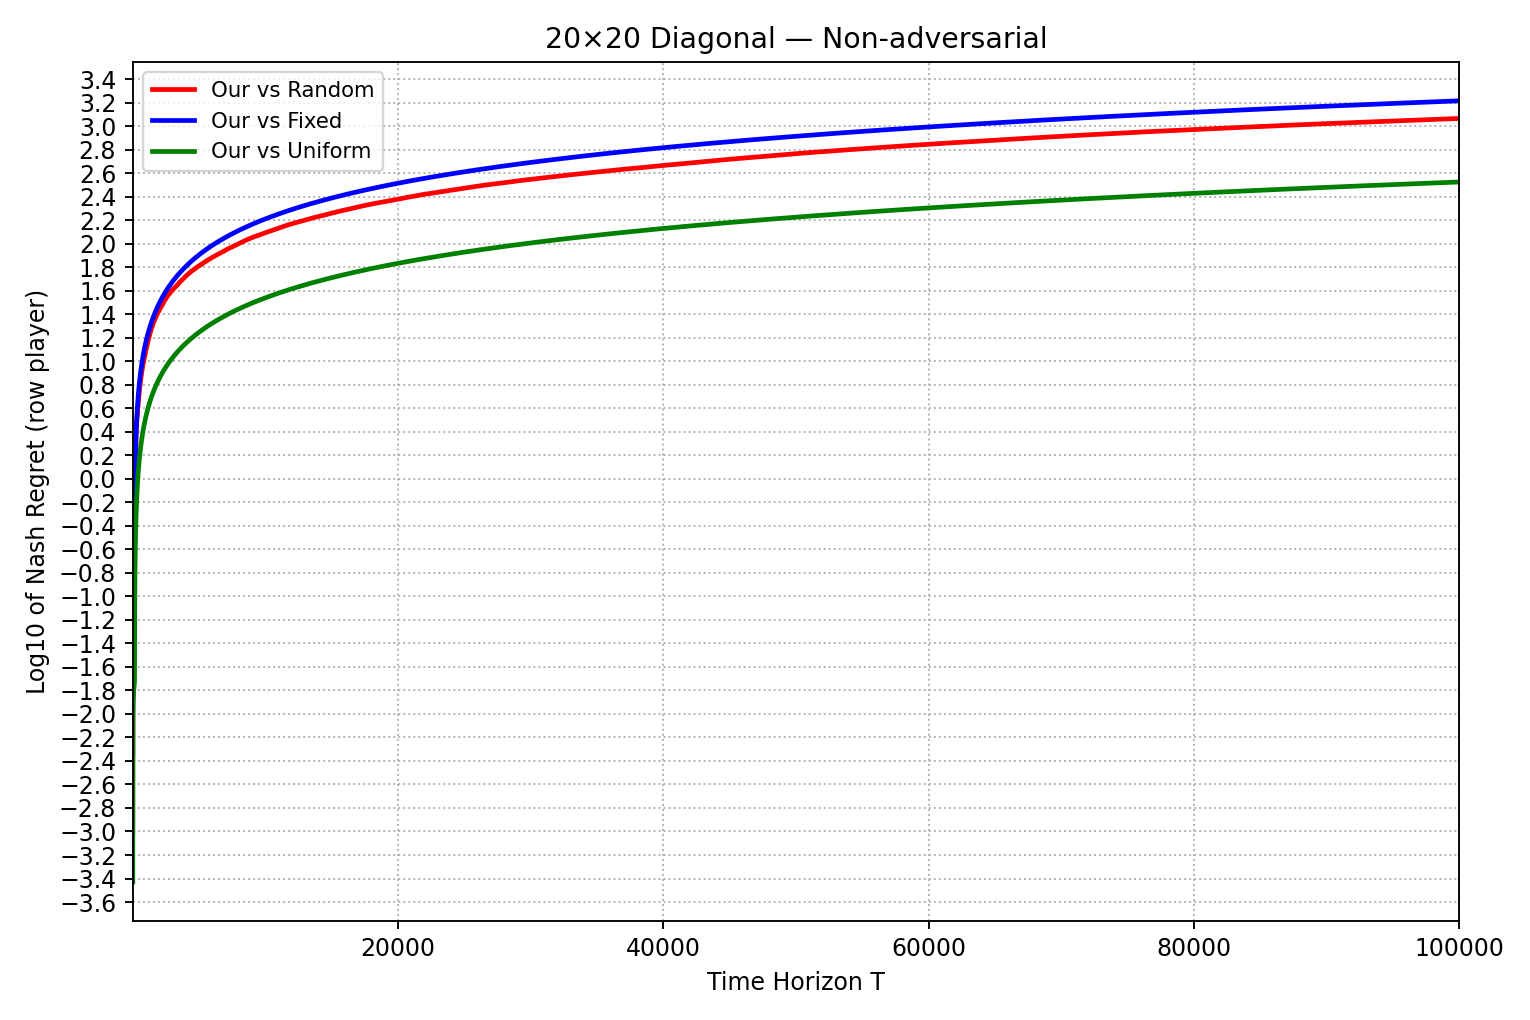
\includegraphics[width=0.78\textwidth]{figures/section3_non-adversarial_paper-lite_n20.png}

  \vspace{0.15cm}
  {\small (a)}

  \vspace{0.40cm}

  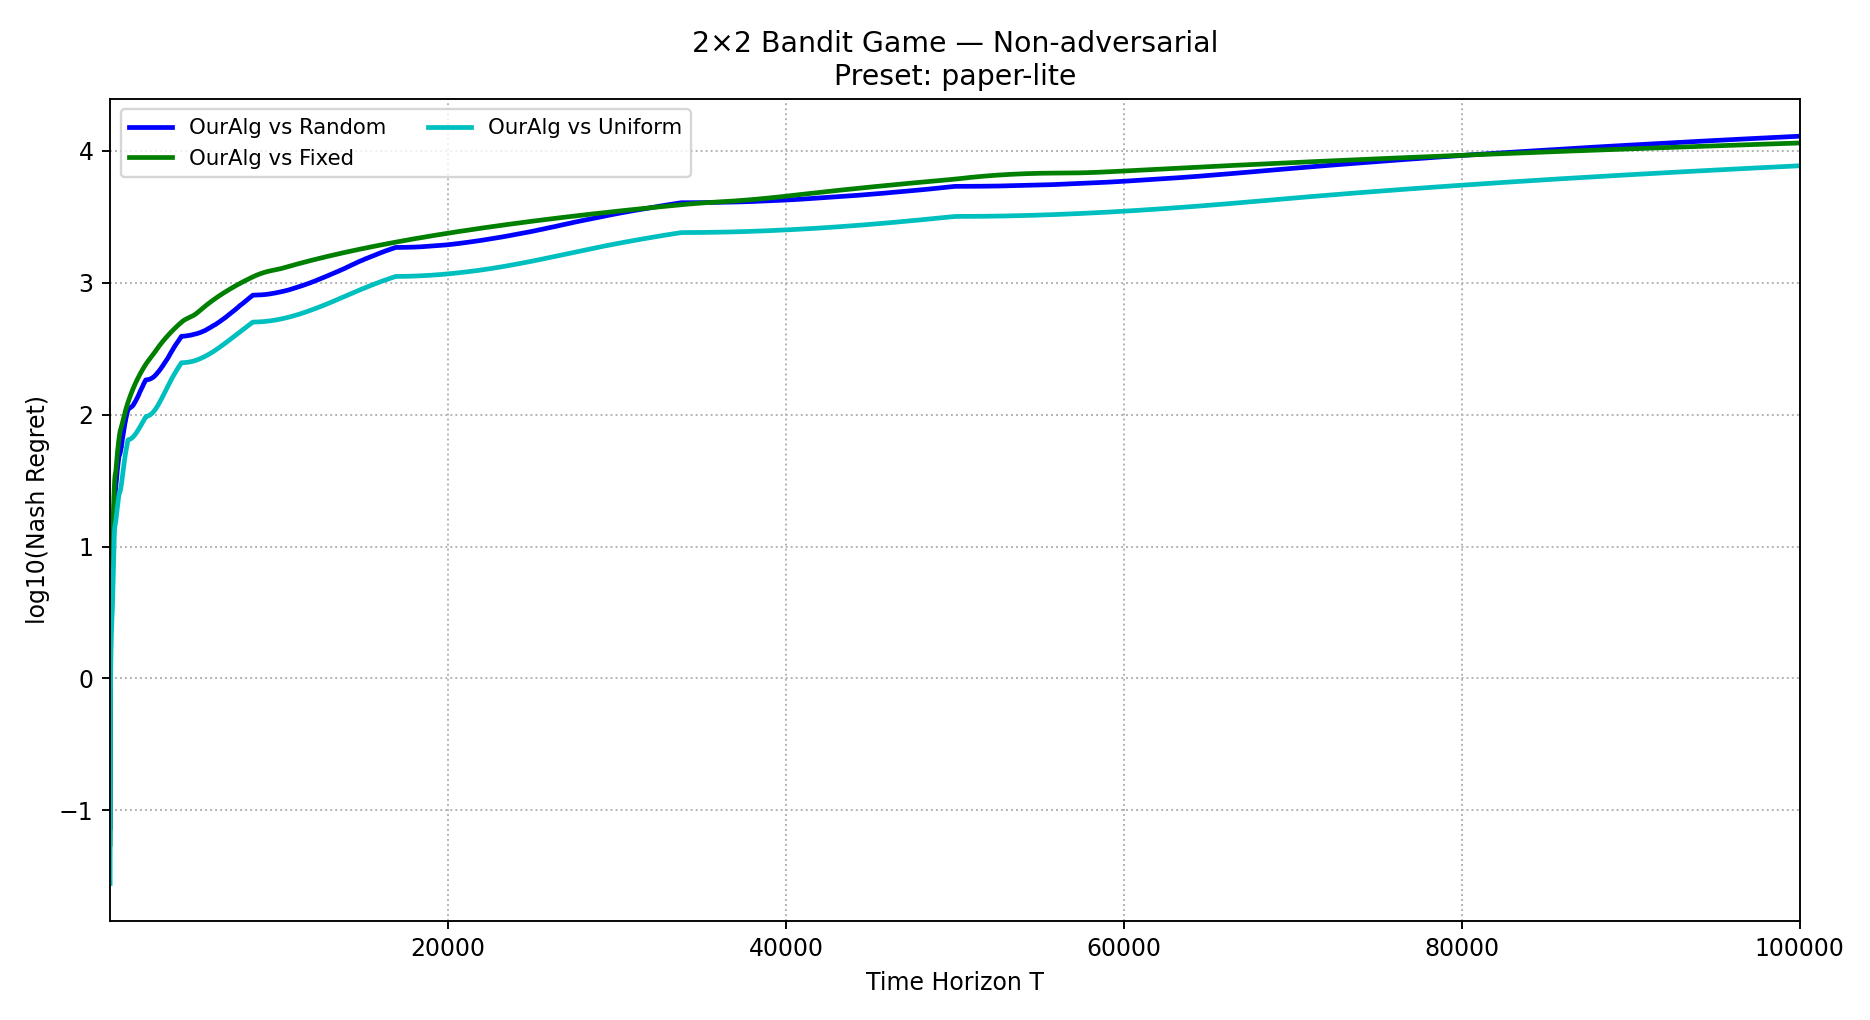
\includegraphics[width=0.88\textwidth]{figures/section4_bilateral_non-adversarial_paper-lite.png}

  \vspace{0.15cm}
  {\small (b)}

  \caption{Row player's incurred regret when playing against a non-adversarial column player: full-information diagonal-game pairings in panel (a), and $2\times2$ bandit pairings in panel (b).}
  \label{fig:non-adversarial}
\end{figure}


\FloatBarrier

\section{Bandit Nash Regret Beyond $2\times2$: Diagnostic Extension}
We applied the paper's Algorithm~6 to larger diagonal bandit games
$(n \in \{2,3,4,5,7,10\})$ with 128 trials and horizons up to
$T = 10^6$. The extension generalizes all algorithmic components like
gradient, strategy update, phase structure, and epoch logic to their
natural $n$-dimensional analogues. However, two implementation choices
optimize for the diagonal game class: the Nash equilibrium and the
$D$ parameter are computed from diagonal entries of the UCB matrix
$F_2$ only, rather than from the full matrix. This is a computational
choice for stability and speed, not a mathematical requirement.


\begin{table}[!htbp]
  \centering
  \small
  \begin{tabular}{rrrrr}
    \toprule
    $n$ & UCB & EXP3 & OurAlg & OurAlg slope \\
    \midrule
    2 & 27.38 & 340.27 & 12.30 & 0.31 \\
    3 & 37.19 & 890.49 & 21.33 & 0.45 \\
    4 & 41.05 & 1557.19 & 40.47 & 0.73 \\
    5 & 43.14 & 2294.43 & 98.32 & 0.73 \\
    7 & 45.07 & 3882.14 & 609.88 & 1.04 \\
    10 & 45.91 & 6449.91 & 6993.62 & 1.07 \\
    \bottomrule
  \end{tabular}
  \caption{Table~4 reports terminal Nash regret at $T = 10^6$ and terminal (final
decade) log--log slope. The terminal slope shows the limiting growth
rate as $T \to \infty$, while the absolute regret comparison against UCB
shows the practical performance boundary.}
  \label{tab:beyond2x2}
\end{table}

Why the diagonal optimization matters. The paper's Algorithm~6 computes
Nash using all entries of the full UCB matrix $F_2 = \hat{B} + \text{bonus}$,
including off-diagonal entries which carry confidence bonuses from
unobserved pairs. For general matrices, these off-diagonal estimates are
signal. For diagonal games, they are pure noise and the true game has zero
off-diagonal entries, so large off-diagonal bonuses distort Nash
estimation during exploration. By computing Nash from diagonal entries
only, we filter this noise and provide the algorithm with cleaner
strategy direction. This is valid for the diagonal game class but does
not transfer to general games. A purist port of Algorithm~6 to general
$n \times n$ games would use full-matrix Nash, lose to UCB earlier than
$n=5$, and directly address the paper's open problem. Our approach
instead shows where failure occurs even under ideal conditions:
exploration coverage degrades from $n=5$ onward, becomes severe by
$n=10$, and prevents extension beyond the proved $2 \times 2$ regime.

\section{Reproducibility and Limitations}

Several assumptions should qualify the conclusions. The report is designed to be reconstructable without needing to inspect the implementation code. The payoff matrices, feedback models, adversary rules, algorithmic baselines, proposed variants, horizons, seeds, numbers of independent runs, game sizes, noise levels, and evaluation metrics are stated in the methodology and extension sections, especially in Table~\ref{tab:settings}. The repository is included as supplementary material for exact execution and figure regeneration, not as a replacement for the methodological description.

First, all results are finite horizon Monte Carlo estimates. Shaded bands in the figures summarize empirical variation across independent runs using standard deviation style summaries where available; we did not bootstrap formal confidence intervals, so the bands should not be read as theorem level confidence statements. Second, no algorithm was selected by tuning on a held out validation problem: the report shows the paper algorithms and standard baselines under fixed settings. Third, Gaussian clipping changes the observation distribution; this is a reasonable bounded payoff model, but it can introduce bias near the boundaries. Finally, copied figures are used only for stable compilation, while the reported settings in the text are sufficient to understand and reconstruct the experiments.

Overall, the reproduction supports the paper's main empirical claims: the proposed algorithms show flatter regret growth than generic online learning baselines in the settings where the theory applies. The extensions show how sensitive that story is to assumptions: explicit noise awareness helps in the full information diagonal game, the original bandit algorithm remains the correct comparison under Section 4's adversaries with noisy observations, bilateral learning changes the opponent model and produces genuinely different dynamics, and larger bandit games expose limitations outside the proved $2\times2$ regime.

\bibliographystyle{alpha}
\bibliography{references}

\end{document}